\documentclass[border=10pt]{standalone}

\usepackage{tikz}
\usepackage{tikzsymbols}
\usetikzlibrary{calc,patterns,shapes.geometric}

\def\centerarc[#1](#2)(#3:#4:#5){\draw[#1] ($(#2)+({#5*cos(#3)},{#5*sin(#3)})$) arc (#3:#4:#5);}

\begin{document}
	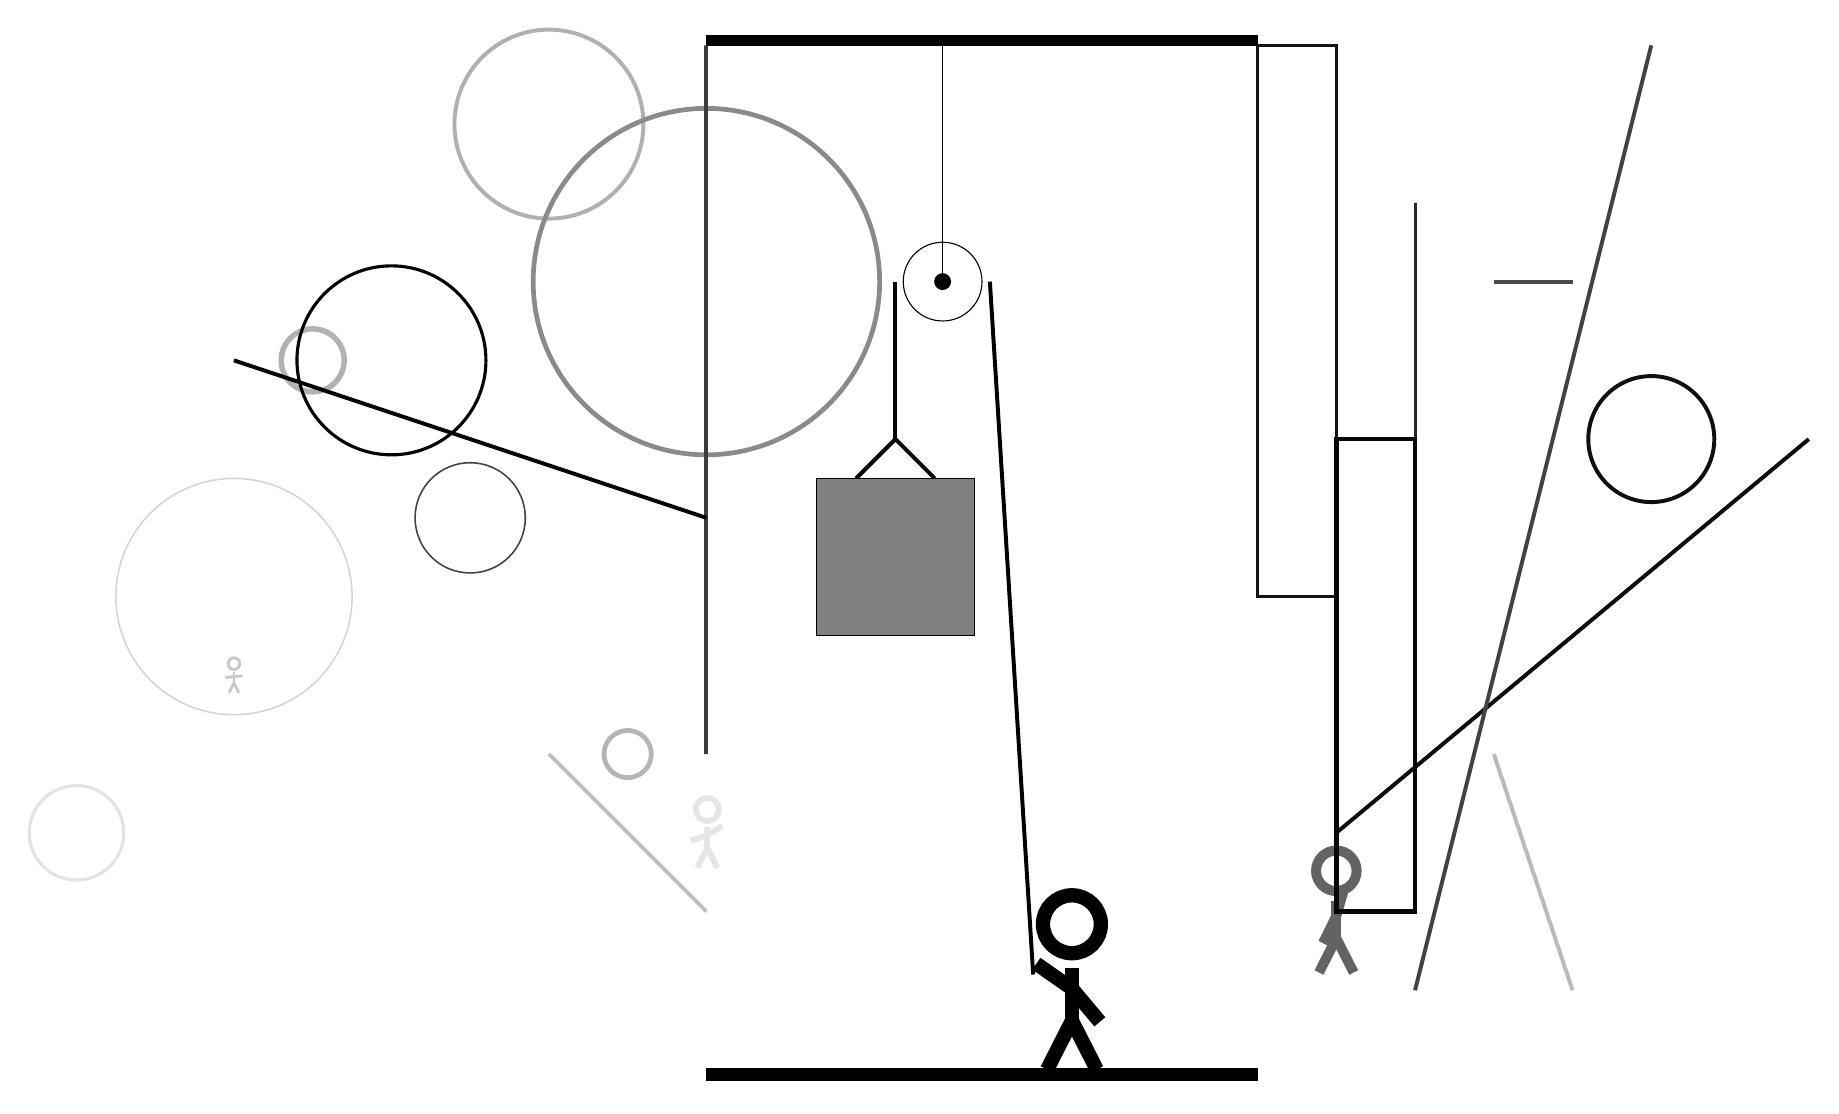
\begin{tikzpicture}
		%%%%% START %%%%%
		
		\draw[fill=black] (-2, 10) rectangle (5, 10.125);
		
		\draw (1, 7) circle (0.5);
		\draw[fill=black] (1, 7) circle (0.1);
		\draw (1, 10) -- (1, 7);
		
		\draw[line width=0.5mm] (-0.1, 4.5) -- (0.4, 5.0) -- (0.9, 4.5);
		\draw[fill=black!50] (-0.6, 4.5) rectangle (1.4, 2.5);
		
		\draw[line width=0.5mm] (0.4, 7) -- (0.4, 5.0);
		\centerarc[line width=0.5mm](1, 7)(0:180:0.6);
		\draw[line width=0.5mm](1.6, 7) -- (2.15, -1.8);
		
		\node at (2.6, -1.9) {\Strichmaxerl[10][-35][-50]};
		
		\node[line width=0.4mm, color=black!61] at (6, -1) {\Strichmaxerl[7][64][74]};
		
		\node[line width=0.7mm, color=black!21] at (-8, 2) {\Strichmaxerl[2][7][5]};
		\draw [line width=0.5mm, color=black!31](-4, 9) circle (1.2);
		\draw[line width=0.5mm, color=black!76](7, 5) -- (7, 1);
		
		\node[line width=0.3mm, color=black!10] at (-2, 0) {\Strichmaxerl[4][18][32]};
		
		\draw [line width=0.2mm, color=black!17](-8, 3) circle (1.5);
		\draw [line width=0.7mm, color=black!30](-7, 6) circle (0.4);
		
		\draw[line width=0.4mm, color=black!85] (7, 8) rectangle (7, 4);
		\draw[line width=0.5mm, color=black!25](-2, -1) -- (-4, 1);
		\draw[line width=0.3mm, color=black!92] (6, 10) rectangle (5, 3);
		\draw [line width=0.3mm, color=black!90](10, -1) circle (0.0);
		\draw[line width=0.5mm, color=black!95](6, 0) -- (12, 5);
		\draw [line width=0.6mm, color=black!46](-2, 7) circle (2.2);
		
		\draw [line width=0.6mm, color=black!29](-3, 1) circle (0.3);
		\draw[line width=0.5mm, color=black!71](9, 7) -- (8, 7);
		\draw [line width=0.2mm, color=black!74](-5, 4) circle (0.7);
		
		\draw[line width=0.5mm, color=black!77] (-2, 10) rectangle (-2, 1);
		\draw[line width=0.5mm, color=black!27](8, 1) -- (9, -2);
		\draw[line width=0.5mm, color=black!74](7, -2) -- (10, 10);
		\draw [line width=0.4mm, color=black!99](-6, 6) circle (1.2);
		\draw[line width=0.5mm, color=black!98](-2, 4) -- (-8, 6);
		
		\draw [line width=0.4mm, color=black!11](-10, 0) circle (0.6);
		
		\draw [line width=0.5mm, color=black!94](10, 5) circle (0.8);
		\draw[line width=0.6mm, color=black!97] (6, -1) rectangle (7, 5);
		
		\draw[fill=black] (-2, -3) rectangle (5, -3.15);
		
		%%%%% END %%%%%
	\end{tikzpicture}
\end{document}